%%%%%%%%%%%%%%%%%%%%%%%%%%%%%%%%%%%%%%%%%
% Promoting Autonomous Navigation THrough Electric Racing (PANTHER) Boat
% SEACAT 2023 Competition Team
% Controls White Paper
%
% Authors:
% Braidan Duffy
%
% Developed using the kaobook LaTeX Template
% Version 1.3 (December 9, 2021)
% For the latest template development version and to make contributions:
% https://github.com/fmarotta/kaobook
%
%%%%%%%%%%%%%%%%%%%%%%%%%%%%%%%%%%%%%%%%%

%----------------------------------------------------------------------------------------
%	PACKAGES AND OTHER DOCUMENT CONFIGURATIONS
%----------------------------------------------------------------------------------------

\documentclass[
	letterpaper, % Page size
	fontsize=10pt, % Base font size
	twoside=true, % Use different layouts for even and odd pages (in particular, if twoside=true, the margin column will be always on the outside)
	%open=any, % If twoside=true, uncomment this to force new chapters to start on any page, not only on right (odd) pages
	%chapterentrydots=true, % Uncomment to output dots from the chapter name to the page number in the table of contents
	numbers=noenddot, % Comment to output dots after chapter numbers; the most common values for this option are: enddot, noenddot and auto (see the KOMAScript documentation for an in-depth explanation)
]{kaobook}

% Choose the language
\ifxetexorluatex
	\usepackage{polyglossia}
	\setmainlanguage{english}
\else
	\usepackage[english]{babel} % Load characters and hyphenation
\fi
\usepackage[english=british]{csquotes}	% English quotes

\usepackage[]{outlines}

\usepackage{color, soul} % Enable text color changes and highlighting

\usepackage{cancel}

\usepackage[]{pdfpages}

\usepackage{diagbox}

% Load packages for testing
% \usepackage{blindtext}
%\usepackage{showframe} % Uncomment to show boxes around the text area, margin, header and footer
%\usepackage{showlabels} % Uncomment to output the content of \label commands to the document where they are used

% Load the bibliography package
\usepackage{kaobiblio}
% \addbibresource{bibliographies/learning_materials.bib} % Learning Materials bibliography file
% \addbibresource{bibliographies/main.bib} % Bibliography file

% Load mathematical packages for theorems and related environments
\usepackage[framed=true]{kaotheorems}

% Load the package for hyperreferences
\usepackage{kaorefs}

\usepackage{authblk}

\usepackage{listings}

\usepackage{xcolor}

\graphicspath{{images/}} % Paths in which to look for images

\makeindex[columns=3, title=Alphabetical Index, intoc] % Make LaTeX produce the files required to compile the index

\makeglossaries % Make LaTeX produce the files required to compile the glossary
\input{glossary.tex} % Include the glossary definitions

\makenomenclature % Make LaTeX produce the files required to compile the nomenclature

% Reset sidenote counter at chapters
%\counterwithin*{sidenote}{chapter}

\usepackage{xcolor}
% \definecolor{codegreen}{rgb}{0,0.6,0}
% \definecolor{codegray}{rgb}{0.5,0.5,0.5}
% \definecolor{codepurple}{rgb}{0.58,0,0.82}
% \definecolor{backcolour}{rgb}{0.95,0.95,0.92}
% \lstdefinestyle{mystyle}{
%     backgroundcolor=\color{backcolour},   
%     commentstyle=\color{codegreen},
%     keywordstyle=\color{blue},
%     numberstyle=\tiny\color{codegray},
%     stringstyle=\color{codepurple},
%     basicstyle=\ttfamily\footnotesize,
%     breakatwhitespace=false,         
%     breaklines=true,                 
%     captionpos=b,                    
%     keepspaces=true,                 
%     numbers=left,                    
%     numbersep=5pt,                  
%     showspaces=false,                
%     showstringspaces=false,
%     showtabs=false,                  
%     tabsize=2
% }
% \lstset{style=mystyle}

%----------------------------------------------------------------------------------------

\begin{document}

%----------------------------------------------------------------------------------------
%	BOOK INFORMATION
%----------------------------------------------------------------------------------------

\titlehead{SEACAT Controls}

\title{SEACAT Controls White Paper}
\subtitle{Version 1.0}

\author[1]{Braidan Duffy \thanks{bduffy2018@my.fit.edu}}
\author[1]{Humberto Lebron-Rivera \thanks{hlebron2020@my.fit.edu}}

\affil[1]{Department of Ocean Engineering and Marine Sciences, Florida Insitute of Technology}

\date{May, 2023}

\publishers{PANTHER Boat Racing Team}

%----------------------------------------------------------------------------------------

\frontmatter % Denotes the start of the pre-document content, uses roman numerals

%----------------------------------------------------------------------------------------
%	OPENING PAGE
%----------------------------------------------------------------------------------------

%\makeatletter
%\extratitle{
%	% In the title page, the title is vspaced by 9.5\baselineskip
%	\vspace*{9\baselineskip}
%	\vspace*{\parskip}
%	\begin{center}
%		% In the title page, \huge is set after the komafont for title
%		\usekomafont{title}\huge\@title
%	\end{center}
%}
%\makeatother

%----------------------------------------------------------------------------------------
%	COPYRIGHT PAGE
%----------------------------------------------------------------------------------------

\makeatletter
\uppertitleback{\@titlehead} % Header

\lowertitleback{
	\textbf{Disclaimer}\\
	Information contained herewithin is compiled from the best efforts of testing and experimentation by the SEACAT controls team.
	It should not be considered final nor fully complete and may contain knowledge gaps throughout.
	Readers intent upon implementing the features discussed within are encouraged to do so, but should not rely on this information.
	\textbf{Programmer's discretion is strongly advised.}
	
	\medskip
	
	\textbf{License}\\
	Copyright 2023 \@author\\

	Permission is hereby granted, free of charge, to any person obtaining a copy of this software and associated documentation files (the “Software”), to deal in the Software without restriction, including without limitation the rights to use, copy, modify, merge, publish, distribute, sublicense, and/or sell copies of the Software, and to permit persons to whom the Software is furnished to do so, subject to the following conditions:

	The above copyright notice and this permission notice shall be included in all copies or substantial portions of the Software.

	THE SOFTWARE IS PROVIDED “AS IS”, WITHOUT WARRANTY OF ANY KIND, EXPRESS OR IMPLIED, INCLUDING BUT NOT LIMITED TO THE WARRANTIES OF MERCHANTABILITY, FITNESS FOR A PARTICULAR PURPOSE AND NONINFRINGEMENT. IN NO EVENT SHALL THE AUTHORS OR COPYRIGHT HOLDERS BE LIABLE FOR ANY CLAIM, DAMAGES OR OTHER LIABILITY, WHETHER IN AN ACTION OF CONTRACT, TORT OR OTHERWISE, ARISING FROM, OUT OF OR IN CONNECTION WITH THE SOFTWARE OR THE USE OR OTHER DEALINGS IN THE SOFTWARE.
	
	\medskip
	
	\textbf{Colophon} \\
	This document was typeset with the help of \href{https://sourceforge.net/projects/koma-script/}{\KOMAScript} and \href{https://www.latex-project.org/}{\LaTeX} using the \href{https://github.com/fmarotta/kaobook/}{kaobook} class.
	
	The source code of this book is available at:\\\url{https://github.com/fmarotta/kaobook}
	
	(You are welcome to contribute!)
	
	\medskip
	
	\textbf{Publisher} \\
	First printed in May 2023 by \@publishers
}
\makeatother

%----------------------------------------------------------------------------------------
%	DEDICATION
%----------------------------------------------------------------------------------------

\dedication{
	\emph{Ab experientia, intellectus}
}

%----------------------------------------------------------------------------------------
%	OUTPUT TITLE PAGE AND PREVIOUS
%----------------------------------------------------------------------------------------

% Note that \maketitle outputs the pages before here

\maketitle

%----------------------------------------------------------------------------------------
%	PREFACE
%----------------------------------------------------------------------------------------

% \input{chapters/preface.tex}
% \index{preface}

%----------------------------------------------------------------------------------------
%	TABLE OF CONTENTS & LIST OF FIGURES/TABLES
%----------------------------------------------------------------------------------------

\begingroup % Local scope for the following commands

% Define the style for the TOC, LOF, and LOT
%\setstretch{1} % Uncomment to modify line spacing in the ToC
%\hypersetup{linkcolor=blue} % Uncomment to set the colour of links in the ToC
\setlength{\textheight}{230\hscale} % Manually adjust the height of the ToC pages

% Turn on compatibility mode for the etoc package
\etocstandarddisplaystyle % "toc display" as if etoc was not loaded
\etocstandardlines % "toc lines" as if etoc was not loaded

\tableofcontents % Output the table of contents

\listoffigures % Output the list of figures

% Comment both of the following lines to have the LOF and the LOT on different pages
\let\cleardoublepage\bigskip
\let\clearpage\bigskip

\listoftables % Output the list of tables

\endgroup

%----------------------------------------------------------------------------------------
%	MAIN BODY
%----------------------------------------------------------------------------------------

\mainmatter{} % Denotes the start of the main document content, resets page numbering and uses arabic numbers
\setchapterstyle{kao} % Choose the default chapter heading style

% ===========================================
% Introduction
% Written by: Braidan Duffy
%
% Date: 05/02/2023
% Last Revision: 05/02/2023
% ============================================

\setchapterstyle{kao}
\chapter{Introduction}
\setchapterpreamble[u]{\margintoc}
\labch{introduction}

The Self-propelled Electric Autonomous CATamaran (SEACAT) is envisioned to compete in the Promoting Electric Propulsion (PEP) competition sponsored by the American Society of Naval Engineers (ASNE).
This is an annual competition that challenges teams from the academic, public, and private sectors to design, build, and race small electric boats in a 5-mile course.
These boats can either be crewed or uncrewed and are tasked with completing the 5 single-mile laps as quickly as possible.

For SEACAT 2023, the requirements for the system are deceptively simple: 1) The vessel must be uncrewed, and 2) the vessel should be able to navigate the course autonomously via GPS waypoints.
These high level requirements drive a variety of lower-level requirements which will be discussed in Section \ref{ssec:requirements}.
For any robotic system, the control systems engineers must balance the requirements of the system with the capabilities and constraints present.
In SEACAT 2023's case, as with many other systems, the largest constraints present are time and cost, and given the limited experience available on the controls team, capabilities also had to be limited.

In this paper, the background, controls architecture, implementation, and testing strategies for SEACAT 2023 will be discussed.
This is intended as both a guide into our implementation of a USV control system, as well as the documentation required as a part of the PEP competition.
In the future, it is expected that this document will be updated to include relevant new information added by future teams.
These editions should be mentioned in the Revision History Table (Table \ref{tab:revision_history}) in the Appendix.

\section{Background} \labsec{background}
This section contains some of the research notes that were compiled during the design of SEACAT 2023's controls system.

\subsection[]{Dynamic Modelling}
One of the first steps in analyzing the control systems for a catamaran is to understand the dynamic relationship it has with the environment and itself.
To accomplish this, we need to perform a couple of steps:

\begin{itemize}
    \item Determine the physical parameters such as its dimensions, mass, and center of gravity. 
    \item Choose a reference frame that will be used to describe the position and orientation of the catamaran. 
    A common choice is an earth-fixed frame, where the x-axis points East, the y-axis points North, and the z-axis points towards space (NEU).
    \item Develop a mathematical model relating the physical parameters and the coordinate frame. 
    This typically involves writing equations of motion that describe the translations and rotational motion of the catamaran. 
    The equations of motion can be derived using techniques such as Lagrangian mechanics or Newton-Euler dynamics.
    \item Model the hydrodynamic forces acting on the catamaran, such as lift, drag, and wave-making resistance. 
    This can be done using empirical models, computational fluid dynamics simulations, or experimental data. 
    Most of this information can be found in reference textbooks.
    \item Incorporate control inputs (e.g. rudder, thruster commands), into the model. 
    These inputs can be modeled as time-varying inputs to the equations of motion.
\end{itemize}

The resulting dynamic model can be used to simulate the motion of the catamaran under various conditions and control inputs. 
This is a part of the "digital twin" and can be used to predict future states of the craft which can be useful for analyzing its stability, performance, and response to external disturbances. \sidenote{The complexity of the dynamic model will depend on the accuracy required and the intended use of the model. Simplified models may be sufficient for some applications, while more complex models may be necessary for others.}

The dynamic model will take the form of a linear, time-invariant (LTI) model expressed in the standard state-equation form.
To derive this model and program it, we must create a representation, discretize it, and then implement and plot its response.
The implementation of this model can be forwarded to more advanced artificial intelligence algorithms like Bayesian Networks or Extended Kalman Filters for filtering and smoothing.

\paragraph*{Model representation:} The LTI model is represented using the standard state-equation form, which expresses the state of the system in terms of the state variables and their derivatives. The state equation is usually expressed as a set of first-order linear differential equations:

\begin{gather} \labeq{lti_start}
    \frac{d\vec{x}}{dt} = A\vec{x} + B\vec{u} \\
    \vec{y} = C\vec{x} + D\vec{u} \\
    \begin{aligned}
        \text{where } & \vec{x} \text{ is the state vector,} \\
                      & t \text{ is time,} \\
                      & A \text{ is the state-transition matrix,} \\
                      & B \text{ is the input-to-state matrix,} \\
                      & \vec{u} \text{ is the control input vector,} \\
                      & \vec{y} \text{ is the state output vector,} \\
                      & C \text{ is the state-to-output matrix, and } \\
                      & D \text{ is the direct-transformation matrix}.
    \end{aligned} \notag
\end{gather}

\paragraph*{Discretization:} To program the response of the LTI model, the continuous-time model needs to be discretized. 
This can be done using techniques such as the forward Euler method, the backward Euler method, or the trapezoidal method. 
The discrete-time state-space representation of the model is given by:

\begin{gather}
    \vec{x}_{n+1} = A \vec{x}_n + B \vec{u}_n \\
    \vec{y}_n = C \vec{x}_n + D \vec{u}_n
\end{gather}
    
\paragraph*{Kalman Filter} We can integrate these equations into a Kalman filter which fuses a process model and a measurement model to estimate the current state of the system and associated uncertainties.
The process model is represented by the state-equation form, while the measurement model is represented by the relationship between the true state of the system and the measurements obtained from sensors.
We can express the latter as:

\begin{gather}
    \vec{z}_n = H\vec{x}_n + \vec{v}_n \\
    \begin{aligned}
        \text{where } &\vec{z}_n \text{ is the current measurement vector,} \\
                      &H \text{ is the observation matrix,} \\
                      &\vec{v}_n \text{ is the current measurement noise vector}
    \end{aligned} \notag
\end{gather}

In a Kalman filter, the gain ($K_n$) is defined by the ratio of estimate and measurement uncertainties and is calculated at every filter cycle.
It broadly describes how much the filter relies on its estimate of the system states versus the measurements from the inputs.
A higher gain indicates a heavier reliance on the measurement and vice versa.
The Kalman gain is bounded by: $0 <= K_n <= 1$ and defined as:

\begin{equation} \labeq{kalman_gain}
    \begin{aligned}
        K_n &= \frac{\text{Estimate Uncertainty}}{\text{Estimate Uncertainty + Measurement Uncertainty}} \\
            &= \frac{p_{n-1}}{p_{n-1} + r_n}
    \end{aligned}
\end{equation}

We can therefore determine a \textit{State Update Equation} that uses this gain to estimate the current system state:

\begin{gather} \labeq{kalman_state_update}
    \begin{aligned}
        \vec{x}_{n} &= \vec{x}_{n-1} + K_n(\vec{z}_n - \vec{x}_{n-1}) \\
                    &= (1-K_n)\vec{x}_{n-1} + K_n \vec{z}_n
    \end{aligned} \\
    \begin{aligned}
        \text{where } &\vec{x}_n \text{ is the current state estimate,} \\
                      &\vec{x}_{n-1} \text{ is the previous state estimate,} \\
                      &K_n \text{ is the current Kalman gain and,} \\
                      &\vec{z_n} \text{ is the current measurement vector}
    \end{aligned} \notag
\end{gather}

\marginnote[-1.5in]{\textbf{Important note:} When measurement uncertainty is very large, and the estimate uncertainty is small, $K_n << 1$, hence big weight to the estimate and small weight to the measurement. When the opposite is true, $K_n -> 1$, meaning a large weight to the measurement and a small weight to the estimate. This is how the Kalman filter can regulate and smooth out noisy data by knowing the uncertainties.}

Now that we have an estimate of the current system state, we can determine the associated uncertainty with it using the \textit{Estimate Uncertainty Update Equation}. \sidenote{Also referred to as the \textit{Covariance Update Equation}.}
The estimate uncertainty should approach (converge) to 0 with each filter iteration as the filter improves its guessing accuracy.
However, if the measurement uncertainty is large (i.e. $K_n << 1$), the estimate uncertainty will converge more slowly.
The opposite is true if the measurement uncertainty is small.
In other words, the more precise your measurements are, the faster the Kalman filter will converge on the best estimate.

\begin{gather} \labeq{kalman_estimate_uncertainty}
    p_{n} = (1-K_n)p_{n-1} \\
    \begin{aligned}
        \text{where } &p_{n} \text{ is the estimate uncertainty at the current state} \\
                      &K_n \text{ is the Kalman gain at the current state} \\
                      &p_{n-1} \text{ is the estimate uncertainty of the previous state}
    \end{aligned} \notag
\end{gather}

Now that we have the current uncertainties, the Kalman filter can also predict the future uncertainties using the \textit{Estimate Uncertainty Extrapolation Equation}. \sidenote{Also referred to as the \textit{Covariance Extrapolation Equation}}
Like with the State Extrapolation Equations, this is done with dynamic models and will be unique to every example.
This future uncertainty is expressed by the variable, $p_{n+1}$

Additionally, there are uncertainties in the system's dynamic model because the real-world does not perfectly match our mathematical assumptions.
Uncertainty is caused by unanticipated changes in the system due to external factors.
This can be drift caused by ocean current, wind blowing a rocket to the side, drag, friction and, even time dilation in extreme cases.
Generally, these uncertainties can be combined into the Process Noise gain denoted by "$q$"
To account for process noise, it must be included in the Estimate Uncertainty Extrapolation Equation:

\marginnote{If the model is not known to be good or is very noisy, we can increase the process noise gain to reduce the lag error.}

\begin{equation}
    p_{n+1} = p_n + q
\end{equation}

In summary: the filter is initialized with a first guess ($\vec{x}_{0}$) and an associated uncertainty ($p_{0}$). \sidenote{These are generally null or the best guess for the starting state.}
These values are passed into the dynamic model equations and the Estimate Uncertainty Extrapolation Equation to predict the state at the first measurement ($\vec{x}_{1}$) and the associated uncertainty ($p_{1}$).
This is shown as Step 0 in Figure \ref{fig:kalman_filter}.
Then, we can take a measurement ($\vec{z}_n$) and record its uncertainty ($r_n$), using the latter to determine the Kalman gain with Equation \ref{eq:kalman_gain}.
We can then estimate the current state value using Equation \ref{eq:kalman_state_update} using the recorded measurement and the Kalman gain.
The current state estimate and its uncertainty can then be outputted from the filter and used in applications; this process is shown as Steps 1, 2a, and 2b in the figure below.
These values are then fed into the dynamic model to predict the next state and estimate the associated uncertainty (Step 3 in the below diagram).
Optionally, these predicted values can be outputted from the model as well, as the application requires.
This process typically repeats at a refresh rate of $\Delta t$ for every measurement where $n$ increments with every iteration.

\begin{figure*}[h!]
    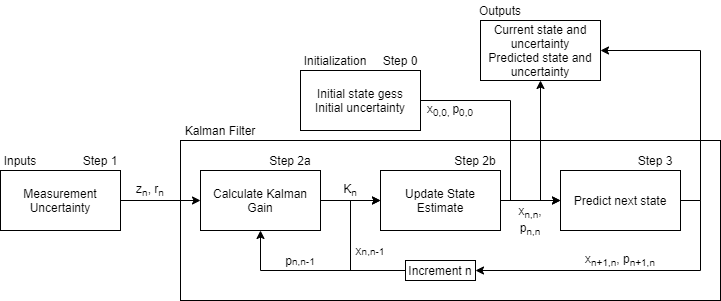
\includegraphics[height=3in]{1_introduction/KalmanFilter.png}
    \caption[Kalman Filter Diagram]{Process diagram for a Kalman filter.}
    \labfig{kalman_filter}
\end{figure*}

\paragraph{Implementation:} The discrete-time state-space representation can be implemented in a programming language, such as Python, C++, or MATLAB, to generate the response of the LTI model to a given input. 
This can be done by updating the state vector at each time step based on the state equation, and computing the output based on the output equation. The input can be specified as a time-varying function or a sequence of values.
Kalman filters are pretty-well documented and understood so multiple libraries in multiple languages exist that already implement the algorithm.

\paragraph*{Plotting the response:} The response of the LTI model can be plotted over time to visualize the behavior of the system. 
This can be useful for analyzing the stability, performance, and robustness of the system, which helps operators tune and diagnose the sensors and models.

% \appendix % From here onwards, chapters are numbered with letters, as is the appendix convention

% \pagelayout{wide} % No margins
% \addpart{Appendix}
% \pagelayout{margin} % Restore margins
% \setchapterstyle{lines}

%----------------------------------------------------------------------------------------

% \backmatter % Denotes the end of the main document content
% \setchapterstyle{plain} % Output plain chapters from this point onwards

%----------------------------------------------------------------------------------------
%	BIBLIOGRAPHY
%----------------------------------------------------------------------------------------

% The bibliography needs to be compiled with biber using your LaTeX editor, or on the command line with 'biber main' from the template directory

% \defbibnote{bibnote}{Here are the references in citation order.\par\bigskip} % Prepend this text to the bibliography
% \printbibliography[heading=bibintoc, title=Bibliography, prenote=bibnote] % Add the bibliography heading to the ToC, set the title of the bibliography and output the bibliography note

%----------------------------------------------------------------------------------------
%	NOMENCLATURE
%----------------------------------------------------------------------------------------

% The nomenclature needs to be compiled on the command line with 'makeindex main.nlo -s nomencl.ist -o main.nls' from the template directory

% \nomenclature{$c$}{Speed of light in a vacuum inertial frame}
% \nomenclature{$h$}{Planck constant}

% \renewcommand{\nomname}{Notation} % Rename the default 'Nomenclature'
% \renewcommand{\nompreamble}{The next list describes several symbols that will be later used within the body of the document.} % Prepend this text to the nomenclature

% \printnomenclature % Output the nomenclature

%----------------------------------------------------------------------------------------
%	GREEK ALPHABET
% 	Originally from https://gitlab.com/jim.hefferon/linear-algebra
%----------------------------------------------------------------------------------------

% \vspace{1cm}

% {\usekomafont{chapter}Greek Letters with Pronunciations} \\[2ex]
% \begin{center}
% 	\newcommand{\pronounced}[1]{\hspace*{.2em}\small\textit{#1}}
% 	\begin{tabular}{l l @{\hspace*{3em}} l l}
% 		\toprule
% 		Character & Name & Character & Name \\ 
% 		\midrule
% 		$\alpha$ & alpha \pronounced{AL-fuh} & $\nu$ & nu \pronounced{NEW} \\
% 		$\beta$ & beta \pronounced{BAY-tuh} & $\xi$, $\Xi$ & xi \pronounced{KSIGH} \\ 
% 		$\gamma$, $\Gamma$ & gamma \pronounced{GAM-muh} & o & omicron \pronounced{OM-uh-CRON} \\
% 		$\delta$, $\Delta$ & delta \pronounced{DEL-tuh} & $\pi$, $\Pi$ & pi \pronounced{PIE} \\
% 		$\epsilon$ & epsilon \pronounced{EP-suh-lon} & $\rho$ & rho \pronounced{ROW} \\
% 		$\zeta$ & zeta \pronounced{ZAY-tuh} & $\sigma$, $\Sigma$ & sigma \pronounced{SIG-muh} \\
% 		$\eta$ & eta \pronounced{AY-tuh} & $\tau$ & tau \pronounced{TOW (as in cow)} \\
% 		$\theta$, $\Theta$ & theta \pronounced{THAY-tuh} & $\upsilon$, $\Upsilon$ & upsilon \pronounced{OOP-suh-LON} \\
% 		$\iota$ & iota \pronounced{eye-OH-tuh} & $\phi$, $\Phi$ & phi \pronounced{FEE, or FI (as in hi)} \\
% 		$\kappa$ & kappa \pronounced{KAP-uh} & $\chi$ & chi \pronounced{KI (as in hi)} \\
% 		$\lambda$, $\Lambda$ & lambda \pronounced{LAM-duh} & $\psi$, $\Psi$ & psi \pronounced{SIGH, or PSIGH} \\
% 		$\mu$ & mu \pronounced{MEW} & $\omega$, $\Omega$ & omega \pronounced{oh-MAY-guh} \\
% 		\bottomrule
% 	\end{tabular} \\[1.5ex]
% 	Capitals shown are the ones that differ from Roman capitals.
% \end{center}

%----------------------------------------------------------------------------------------
%	GLOSSARY
%----------------------------------------------------------------------------------------

% The glossary needs to be compiled on the command line with 'makeglossaries main' from the template directory

% \setglossarystyle{listgroup} % Set the style of the glossary (see https://en.wikibooks.org/wiki/LaTeX/Glossary for a reference)
% \printglossary[title=Special Terms, toctitle=List of Terms] % Output the glossary, 'title' is the chapter heading for the glossary, toctitle is the table of contents heading

%----------------------------------------------------------------------------------------
%	INDEX
%----------------------------------------------------------------------------------------

% The index needs to be compiled on the command line with 'makeindex main' from the template directory

% \printindex % Output the index

%----------------------------------------------------------------------------------------
%	BACK COVER
%----------------------------------------------------------------------------------------

% If you have a PDF/image file that you want to use as a back cover, uncomment the following lines

%\clearpage
%\thispagestyle{empty}
%\null%
%\clearpage
%\includepdf{cover-back.pdf}

%----------------------------------------------------------------------------------------

\end{document}
